\documentclass[../report.tex]{subfiles}
\graphicspath{{\subfix{../image/}}}

\begin{document}
\subsection{Analysis of Dynamics of the Forklift and Motor Sizing}
The forklift required extensive calculations regarding the dynamics and the motor sizing.
These had to be done not only for choosing the right, strong
enough motors, but also for safety and design decisions. How strong can the vehicle accelerate
without tipping over (backwards, forward, fork up and down)? How heavy can it be and where should 
the counterweight be placed? All these questions also determine the dimensioning of the forklift.
The model on which the calculations are based mirrors the design discussed above. It is shown in the 
figure below:
\begin{figure}[H]
    \centering
    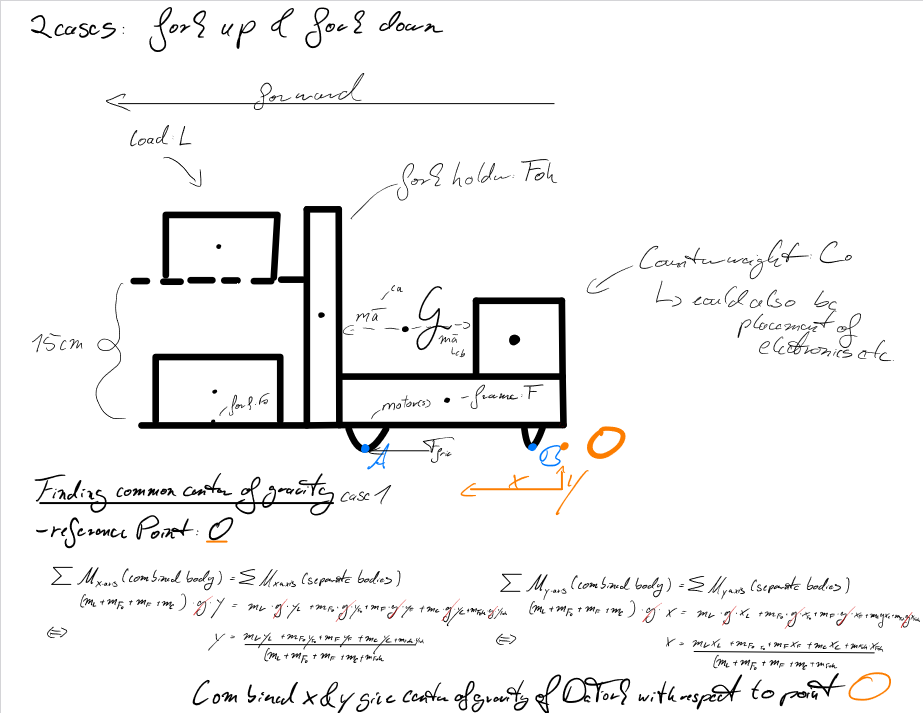
\includegraphics[width=0.25\linewidth]{DaFork.png}
    \caption{Model for calculations}
\end{figure} 
The calculations in the sense of the engineering method where implemented 
in MATLAB live scripts. With this the design process was facilitated. The
exact calculations can be found here: \url{https://github.com/Boti21/SDU-SPRO3-FILES/tree/main/02_Design%20Management}
Consequently, the knowledge obtained in MECH-2 could be brought into praxis.

\end{document}
